\chapter{Тест}
\section{Введение в теорию автоматического управления}
На рубеже XVIII-XIX веков в эпоху промышленного переворота в Европе начинается новый этап развития автоматики, связанный с внедрением ее в промышленность. 1765 год знаменуется постройкой регулятора уровня котла паровой машины И.И. Ползунова. В 1784 го-ду появляется центробежный регулятор скорости паровой машины Дж.Уатта.

В это время формируется ряд важных принципов автоматики: принцип регулирования по отклонению Ползунова - Уатта и принцип регулирования по нагрузке Понселе. Первый из них развился в концепцию обратной связи, второй - в теорию инвариантности (Г.В. Щи-панов, Н.Н. Лузин, Б.Н. Петров). Идея регулирования по нагрузке может быть проиллюстрирована на примере генератора с последова-тельным (сериесным) возбуждением (рис.~\ref{fig:regpovozmusheniu}). При изменении нагрузки меняется ток возбуждения, который соответствующим изменением магнитного потока компенсирует дополнительное падение напряжения на внутреннем сопротивлении якоря генератора. Однако если при этом по каким-либо причинам изменяется скорость вращения якоря генератора, то застабилизировать напряжение на нагрузке в этой схеме уже не удается.

\begin{figure}[h]
	\centering
	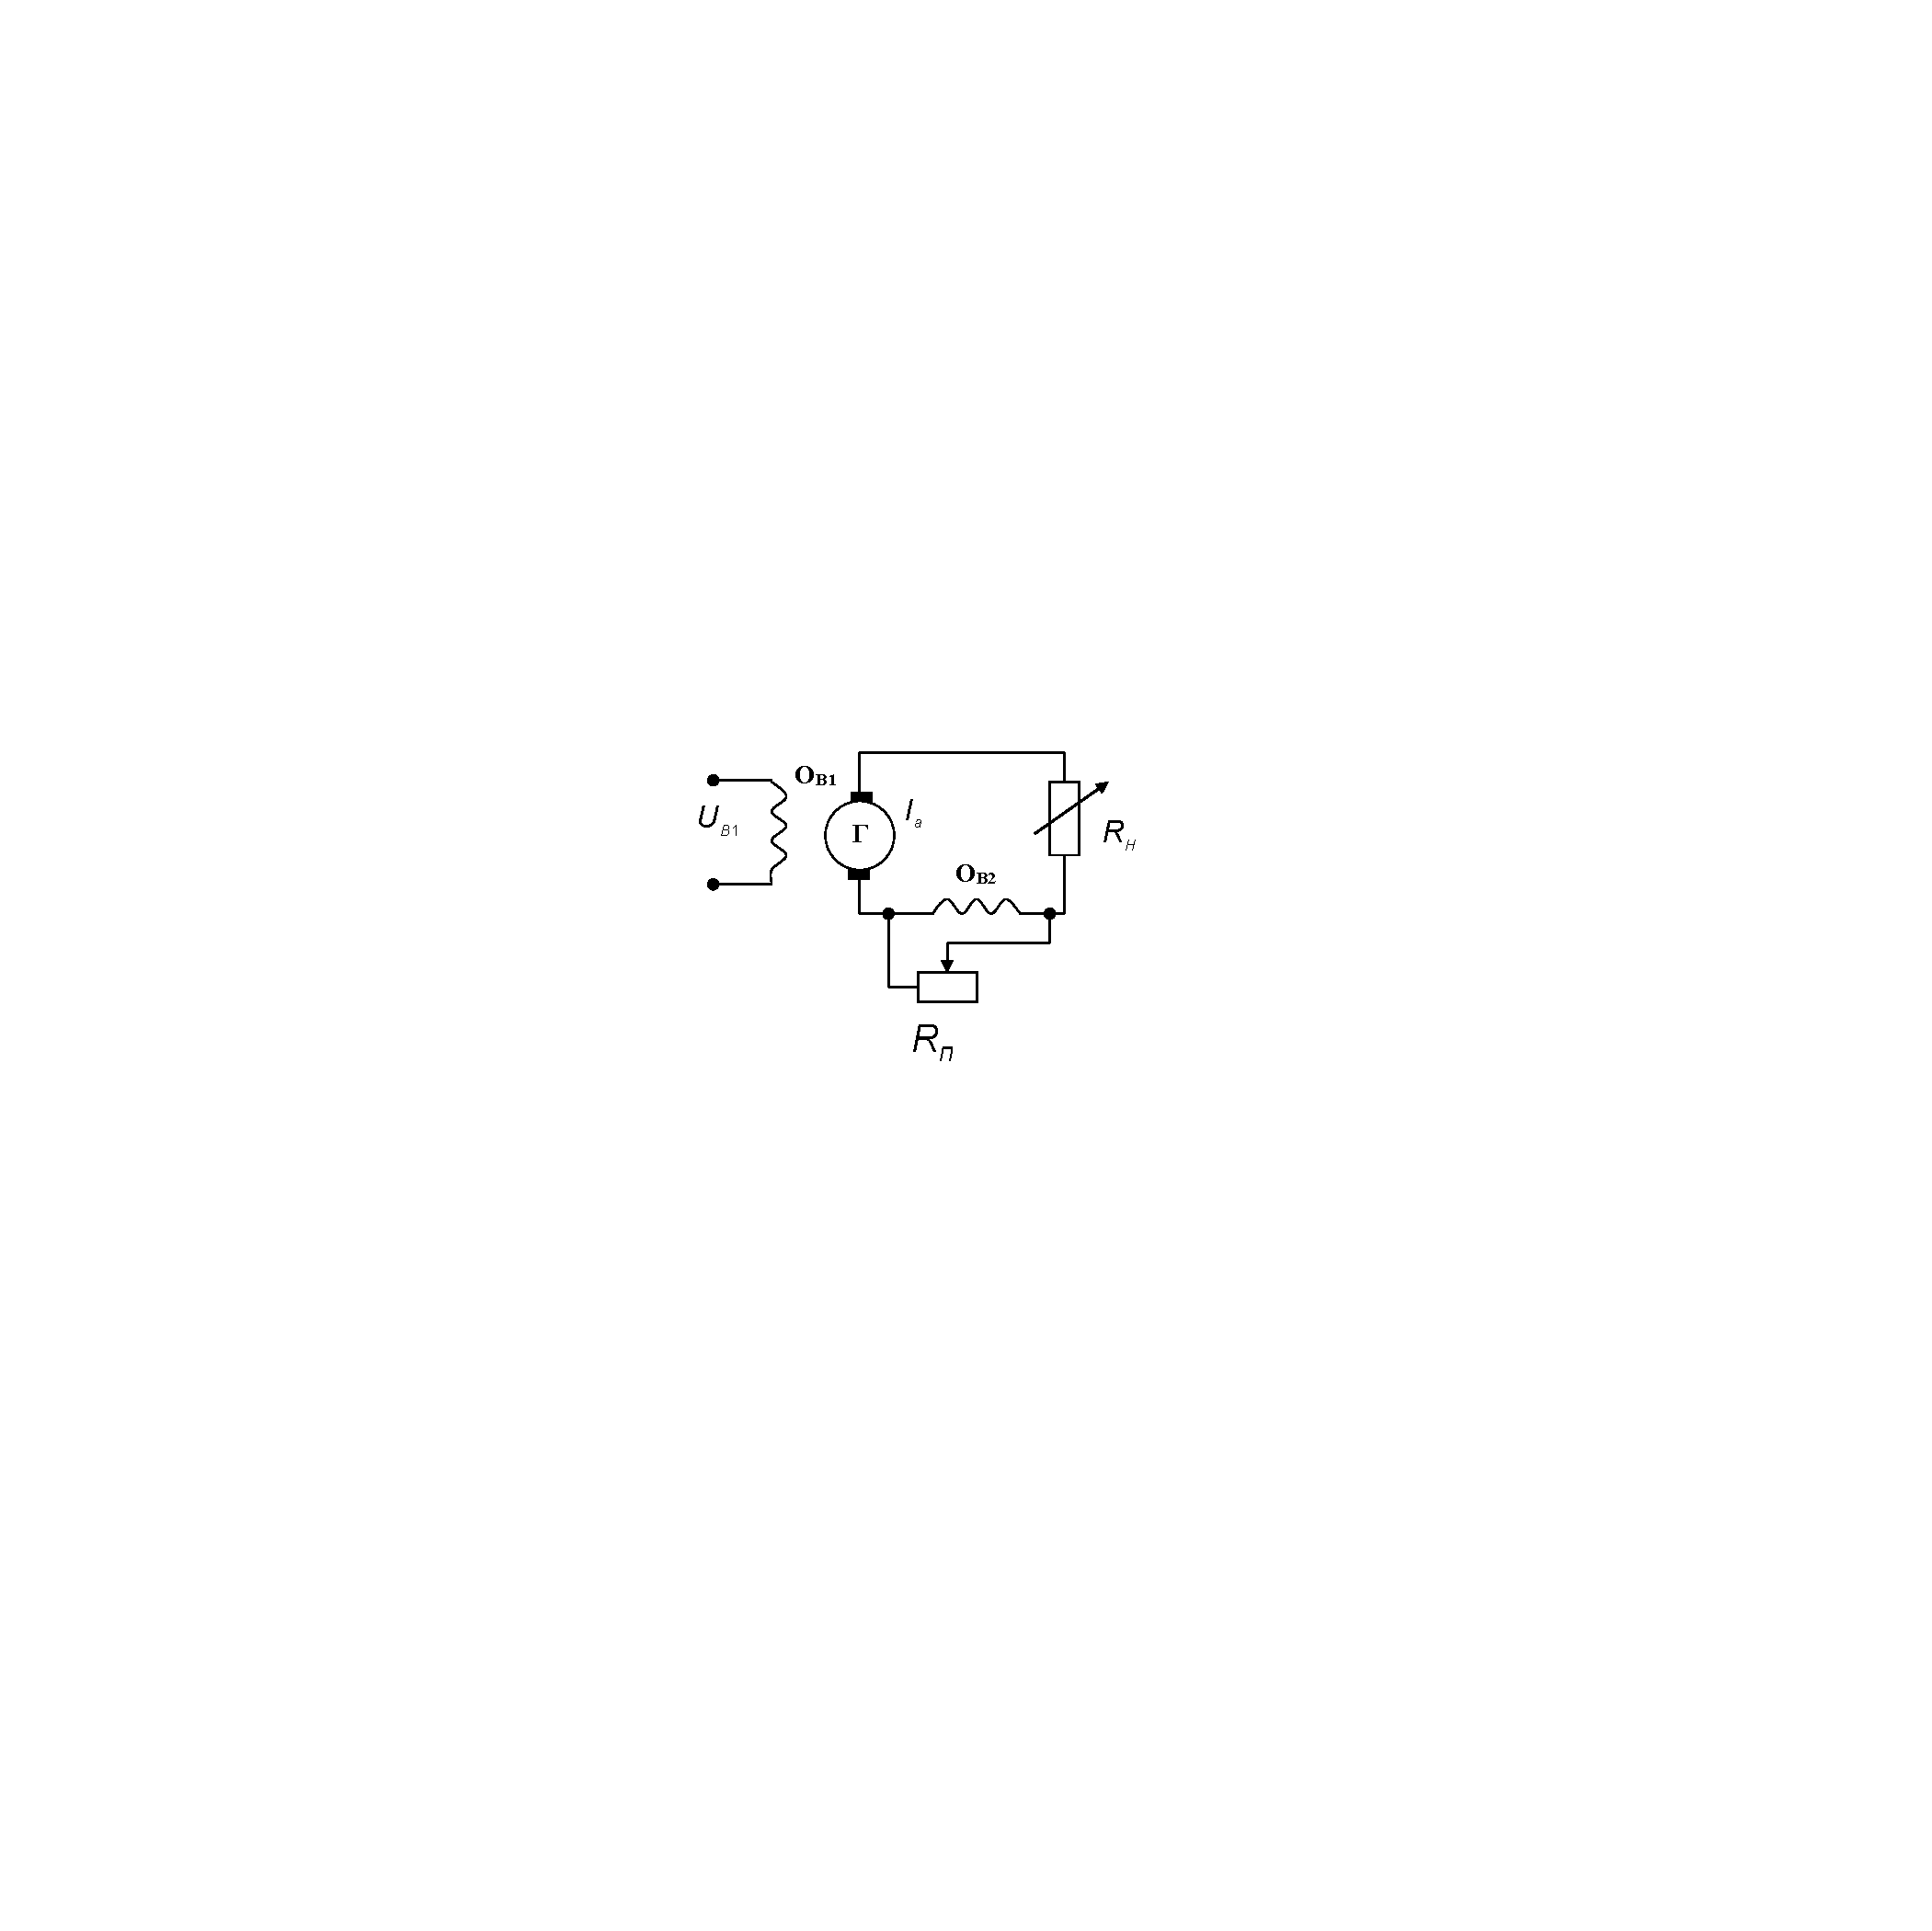
\includegraphics[scale=0.95]{images/RegPoVozmusheniu}
	\caption{Пример регулирования по возмущению }
	\label{fig:regpovozmusheniu}
\end{figure}

От этого недостатка свободна схема, приведенная на рис.~\ref{fig:stabilizaciyanapryazenia} - именно вследствие использования принципа обратной связи. В этой схеме входной потенциометр служит для задания (коэффициент ) величины стабилизируемого напряжения; потенциометр, подключенный к якорю генератора, позволяет регулировать коэффициент об-ратной связи . В этом случае, в отличие от систем регулирования по возмущению, не важно, какая именно причина вызвала изменение регулируемой величины. При изменении напряжения на щётках генератора в соответствии с электрической схемой изменяется напряжение на обмотке возбуждения. При отрицательном знаке обратной связи знак приращения напряжения возбуждения противоположен знаку изменения напряжения якоря генератора. В итоге результирующая величина отклонения напряжения генератора уменьшается по сравнению с соответствующим уходом напряжения в системе без обратной связи. 

\begin{figure}[h]
	\centering
	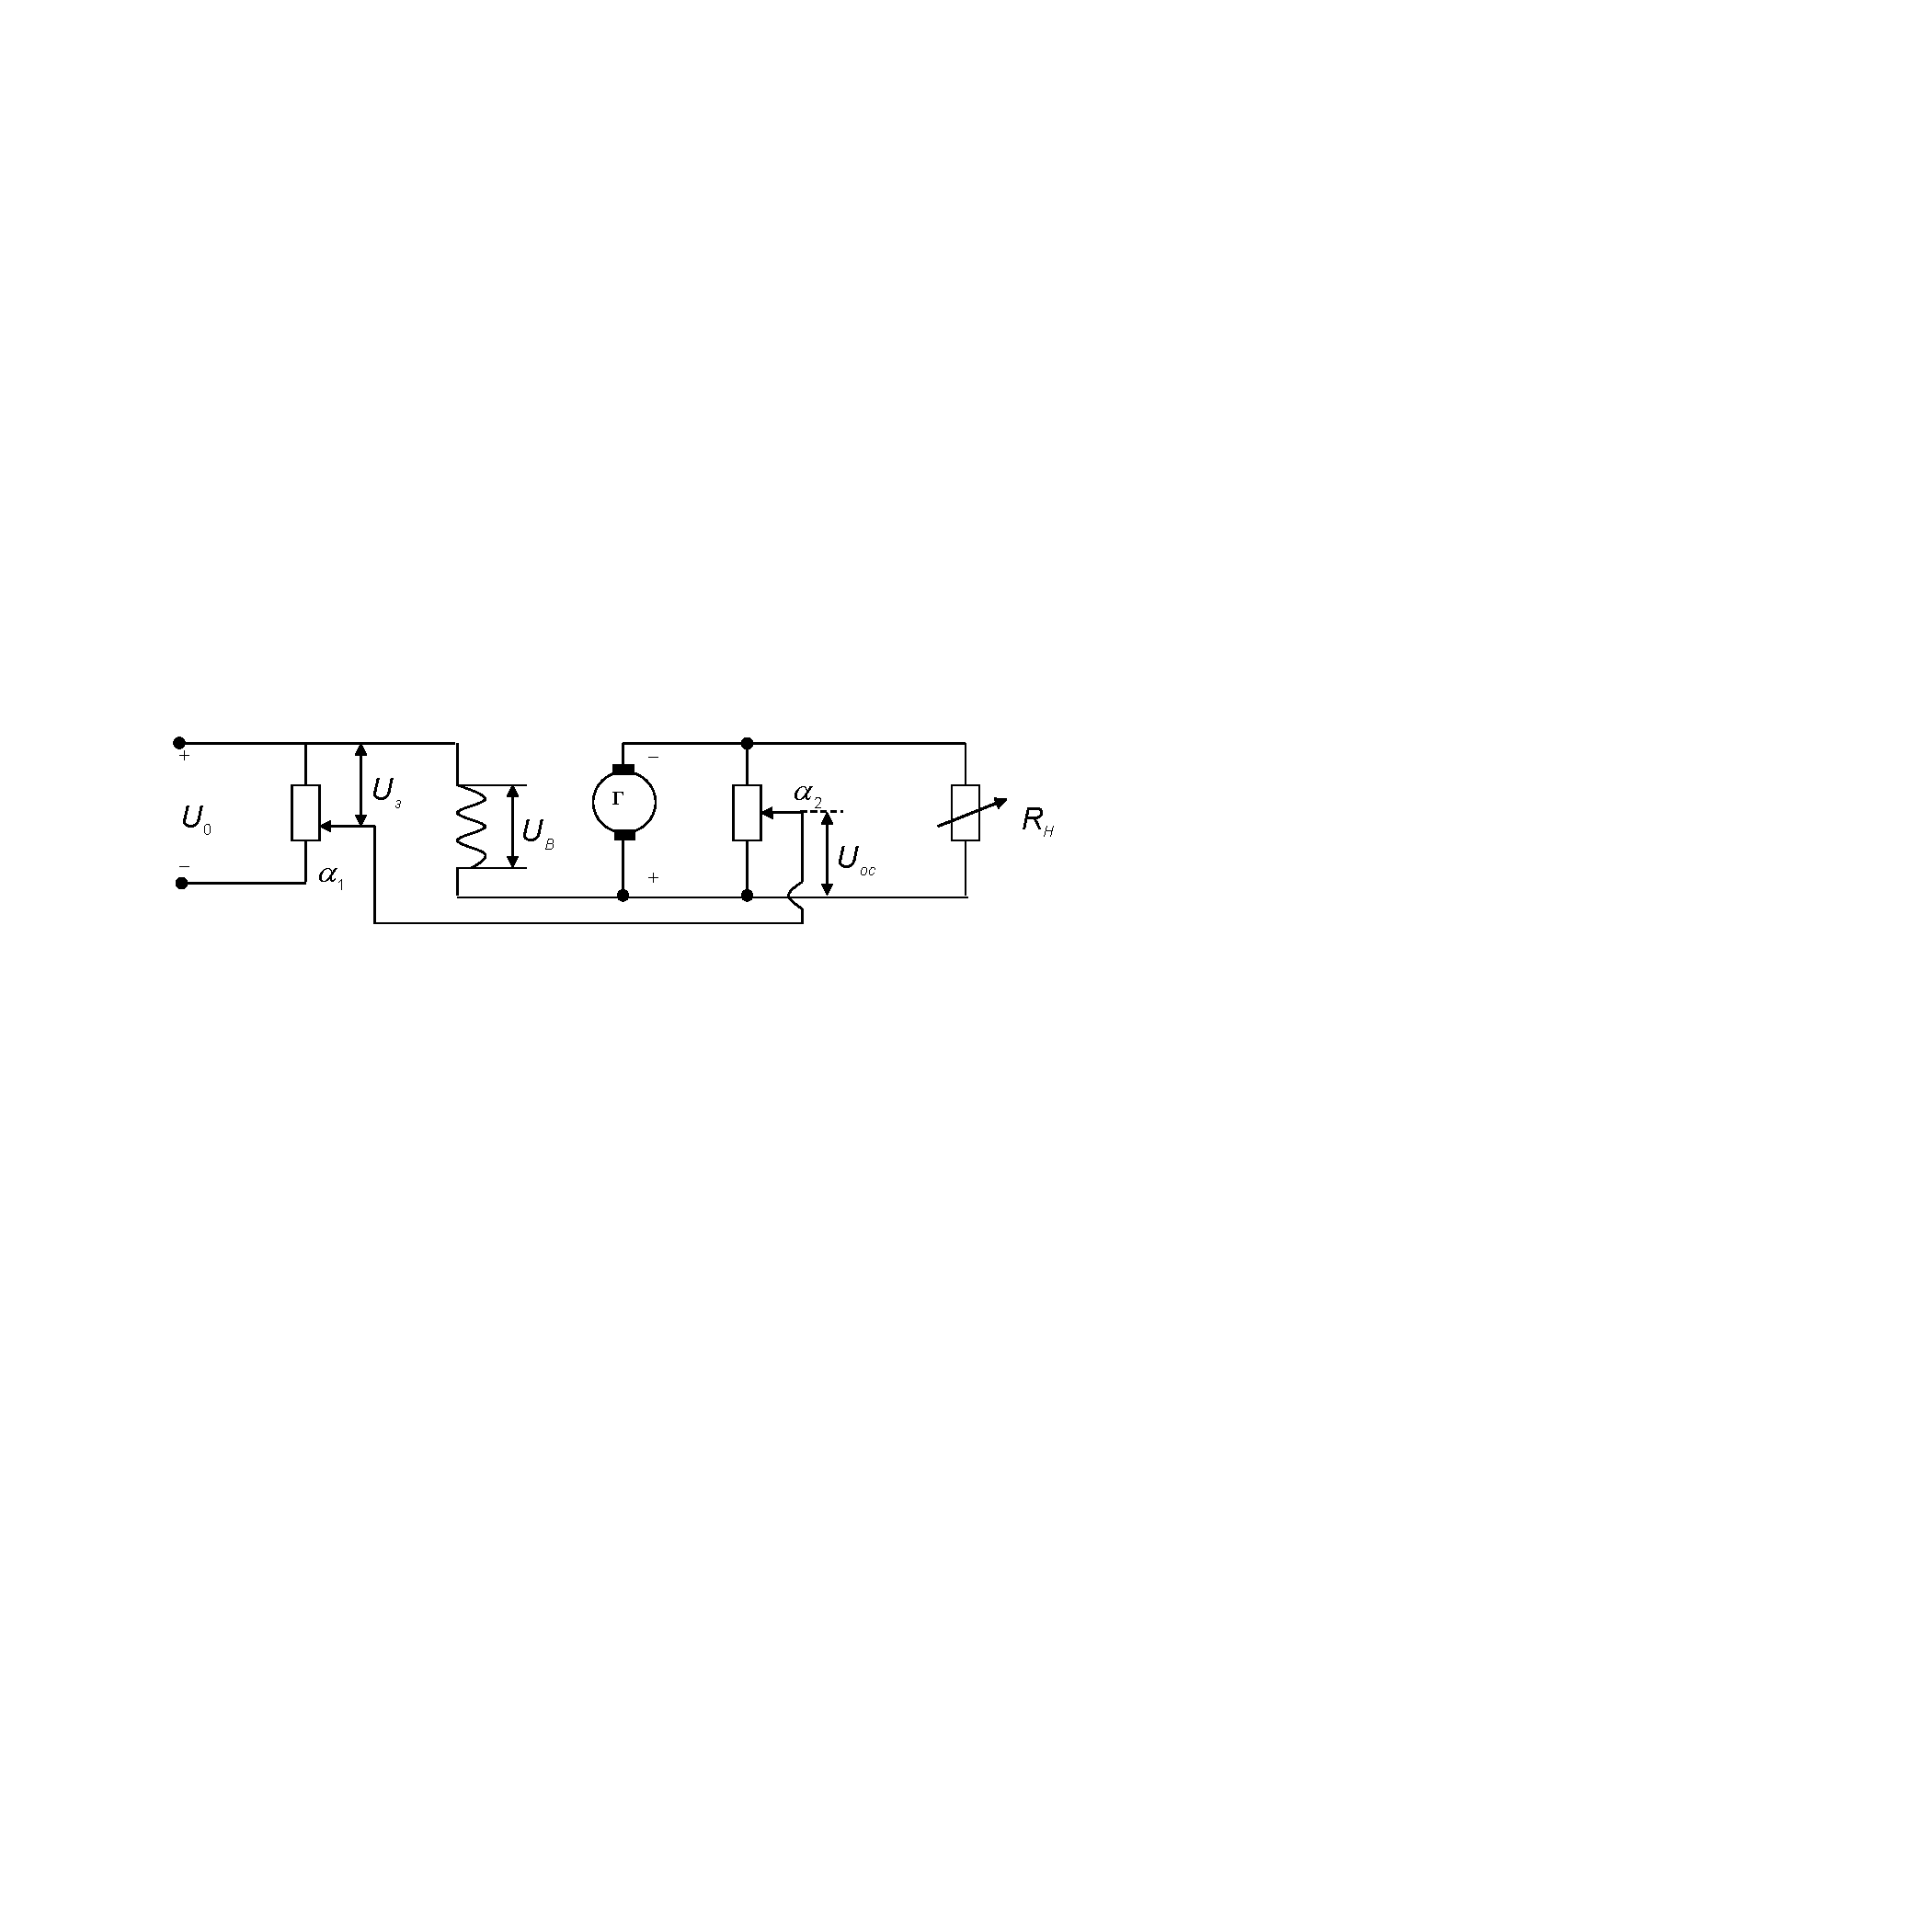
\includegraphics[scale=0.95]{images/StabilizaciyaNapryazenia}
	\caption{Стабилизация напряжения генератора с использованием обратной связи}
	\label{fig:stabilizaciyanapryazenia}
\end{figure}

На этом же принципе построена приведенная на рис.~\ref{fig:steammashine} система стабилизации скорости паровой машины Уатта. На рис.\ref{fig:functionstabilization} представ-лена её функциональная схема. В данной системе с увеличением нагрузочного момента $ M_{Н} $ падают обороты турбины $ \omega $, что приводит к уменьшению расстояния $ 2r $между грузиками центробежного регулятора. Вследствие этого заслонка поднимается (увеличивается расстояние $ S $) и растет расход пара $ Q $ , подаваемого в турбину. Это приводит к росту числа оборотов турбины $ \omega $ а следовательно, к компенсации нагрузочного момента $ M_{Н} $

При изменении нагрузки на валу паровой машины после окончания переходных процессов сохраняется так называемая статическая ошибка. Если бы это было не так, то грузики центробежного регулятора, а вместе с ними и заслонка заняли бы своё первоначальное положение, и не изменившееся в результате количество подаваемого в турбину пара не смогло бы уравновесить изменившийся момент нагрузки. Такая система называется статической. Работа её осуществляется именно за счёт наличия \textit{статической} ошибки. 

Рассматриваемая система относится к классу систем \textit{прямого} действия, то есть таких, в которых для реализации регулятора не ис-пользуются дополнительные источники энергии. В данном случае это плохо, потому что для мощных установок перемещение тяжёлой заслонки потребует неразумно громоздкого и тяжёлого центробежного регулятора.

\begin{figure}[h!]
	\centering
	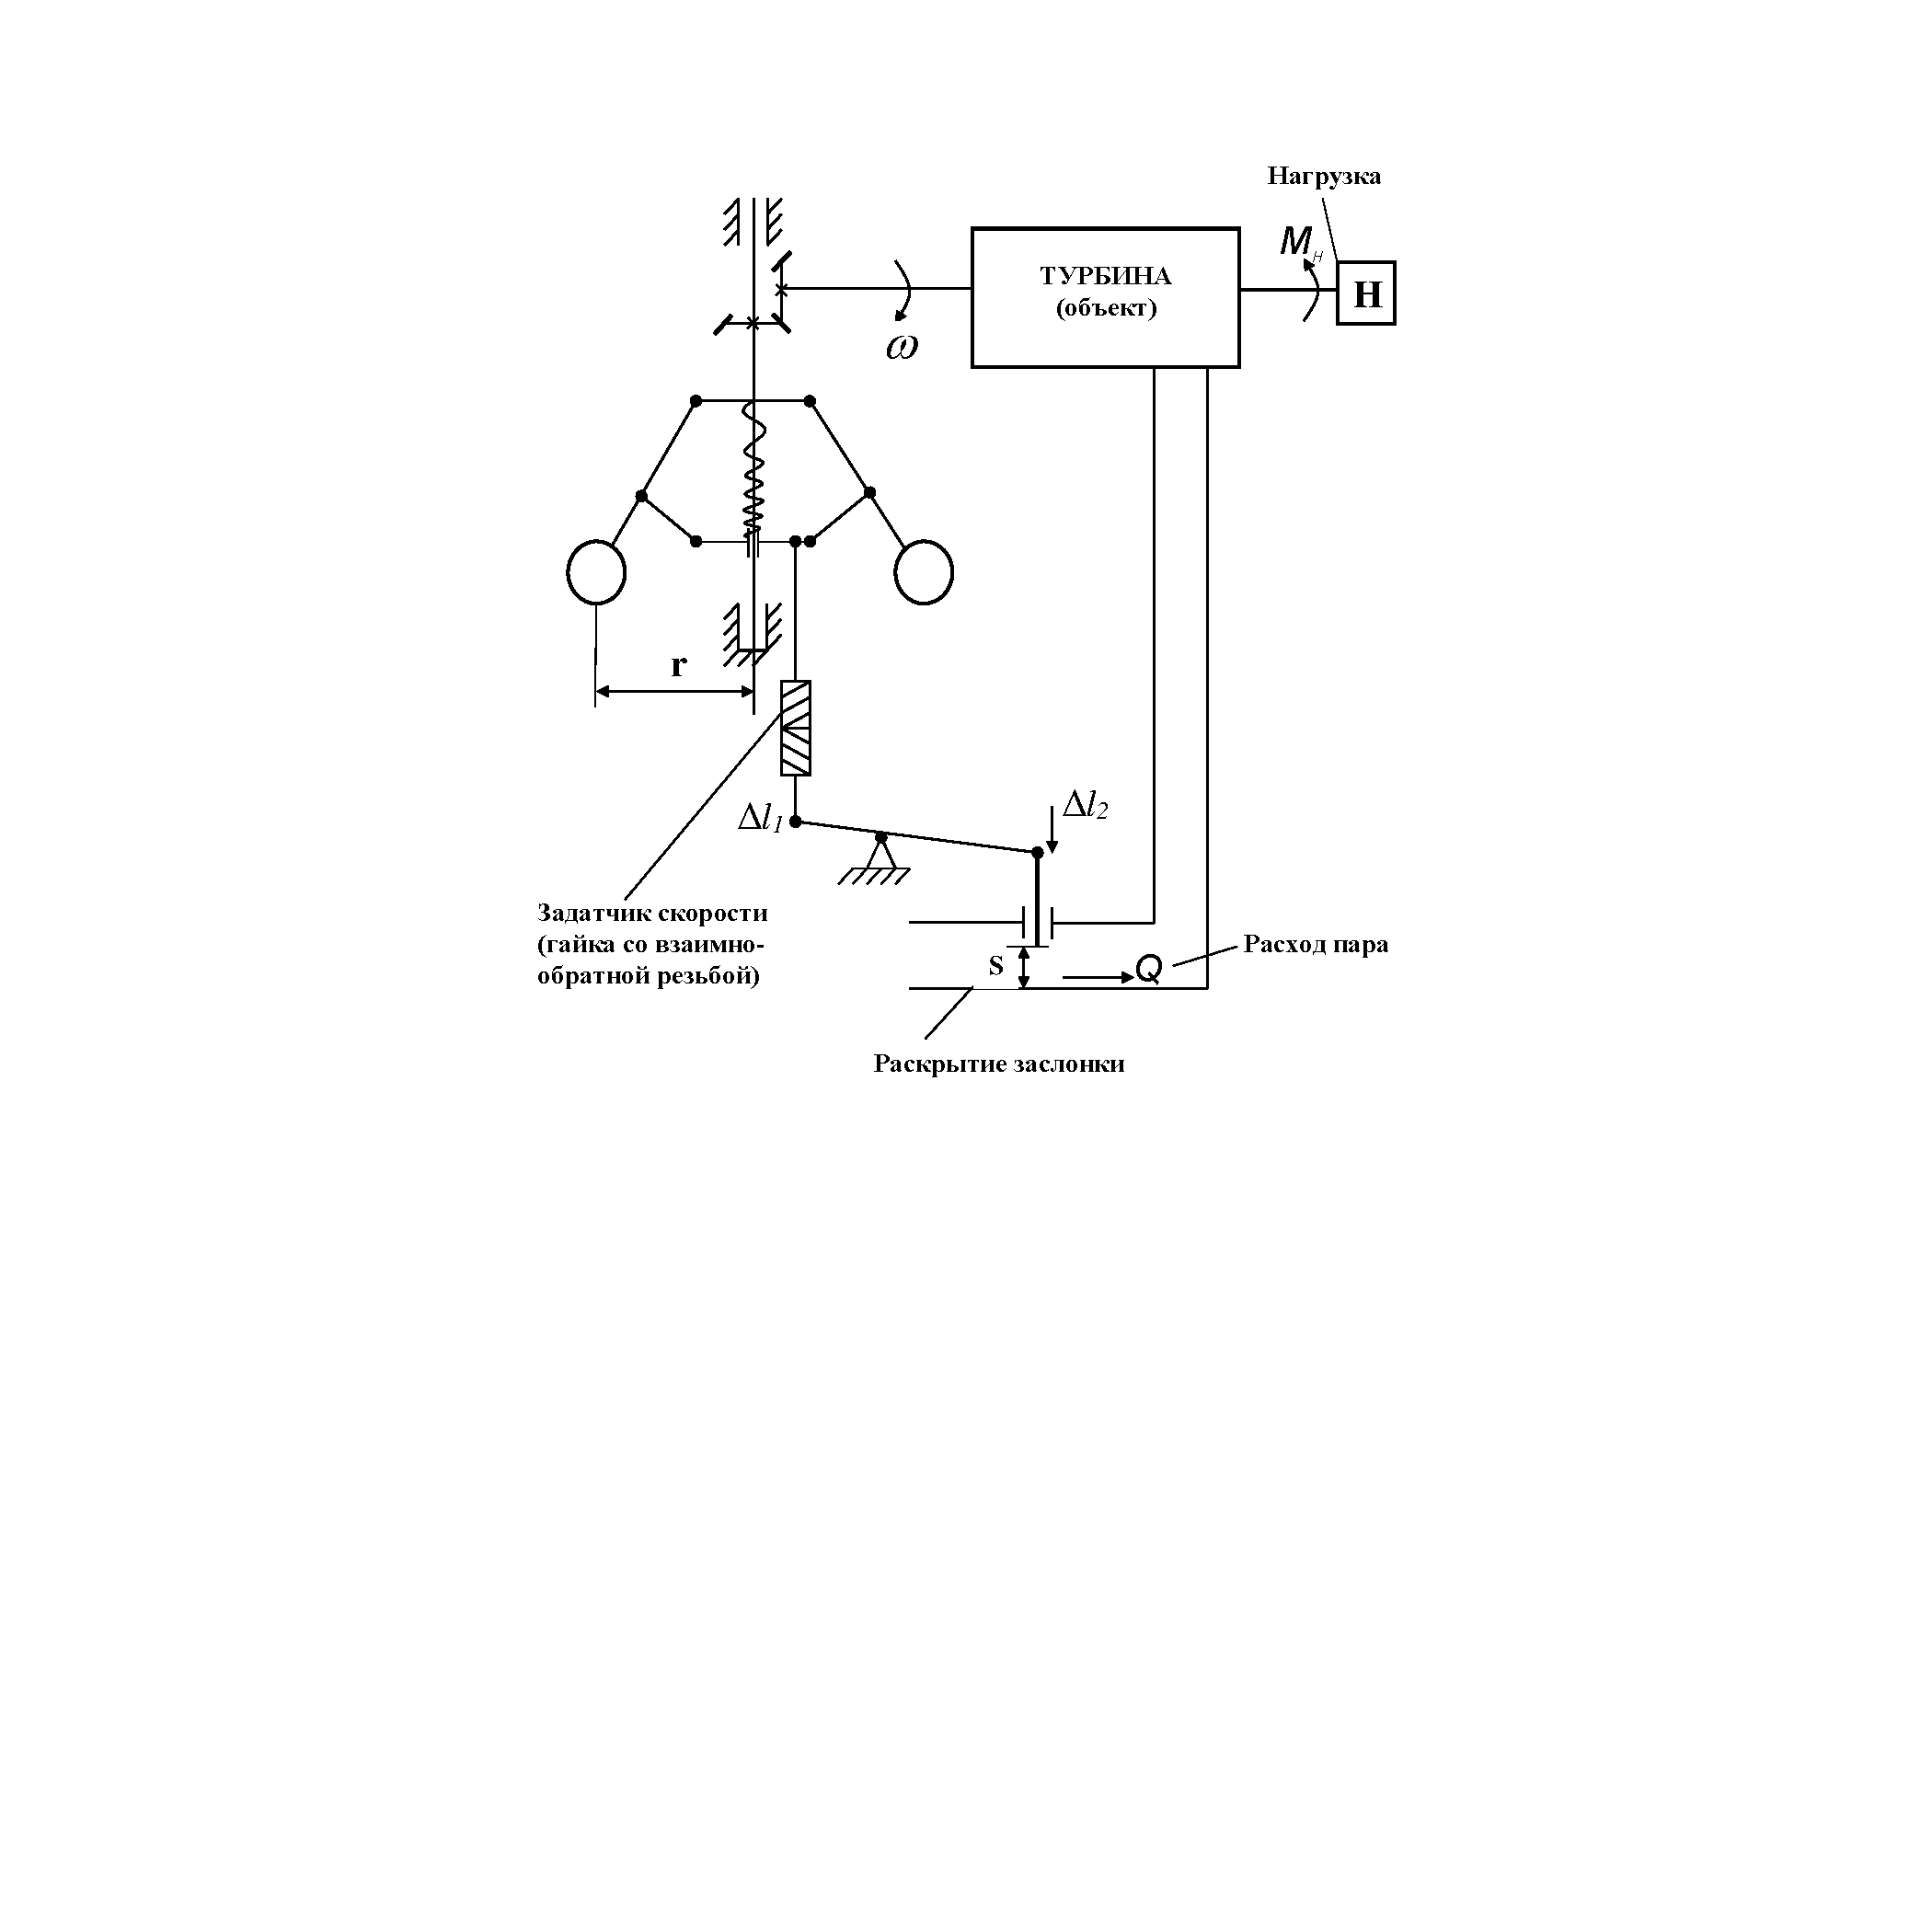
\includegraphics[scale=0.95]{images/SteamMashine}
	\caption{Система стабилизации скорости правой машины }
	\label{fig:steammashine}
\end{figure}

Таким образом, система является статической системой прямого действия.

Введём следующие определения:
\begin{description}
	\item[статистической системой] называют систему, работающую за счет статической ошибки;
	\item[системой прямого действия] называют систему, регулятор которой не имеет собственных источников энергии.
	\item[структурной схемой] называется блок-схема, каждый элемент которой отображает некоторый математический оператор (группу операторов), описывающий рассматриваемую систему.
\end{description}

Использование функциональных и структурных схем позволяет более наглядно представить взаимосвязь между отдельными основными и промежуточными переменными объектов и систем управления

\begin{figure}[h!]
	\centering
	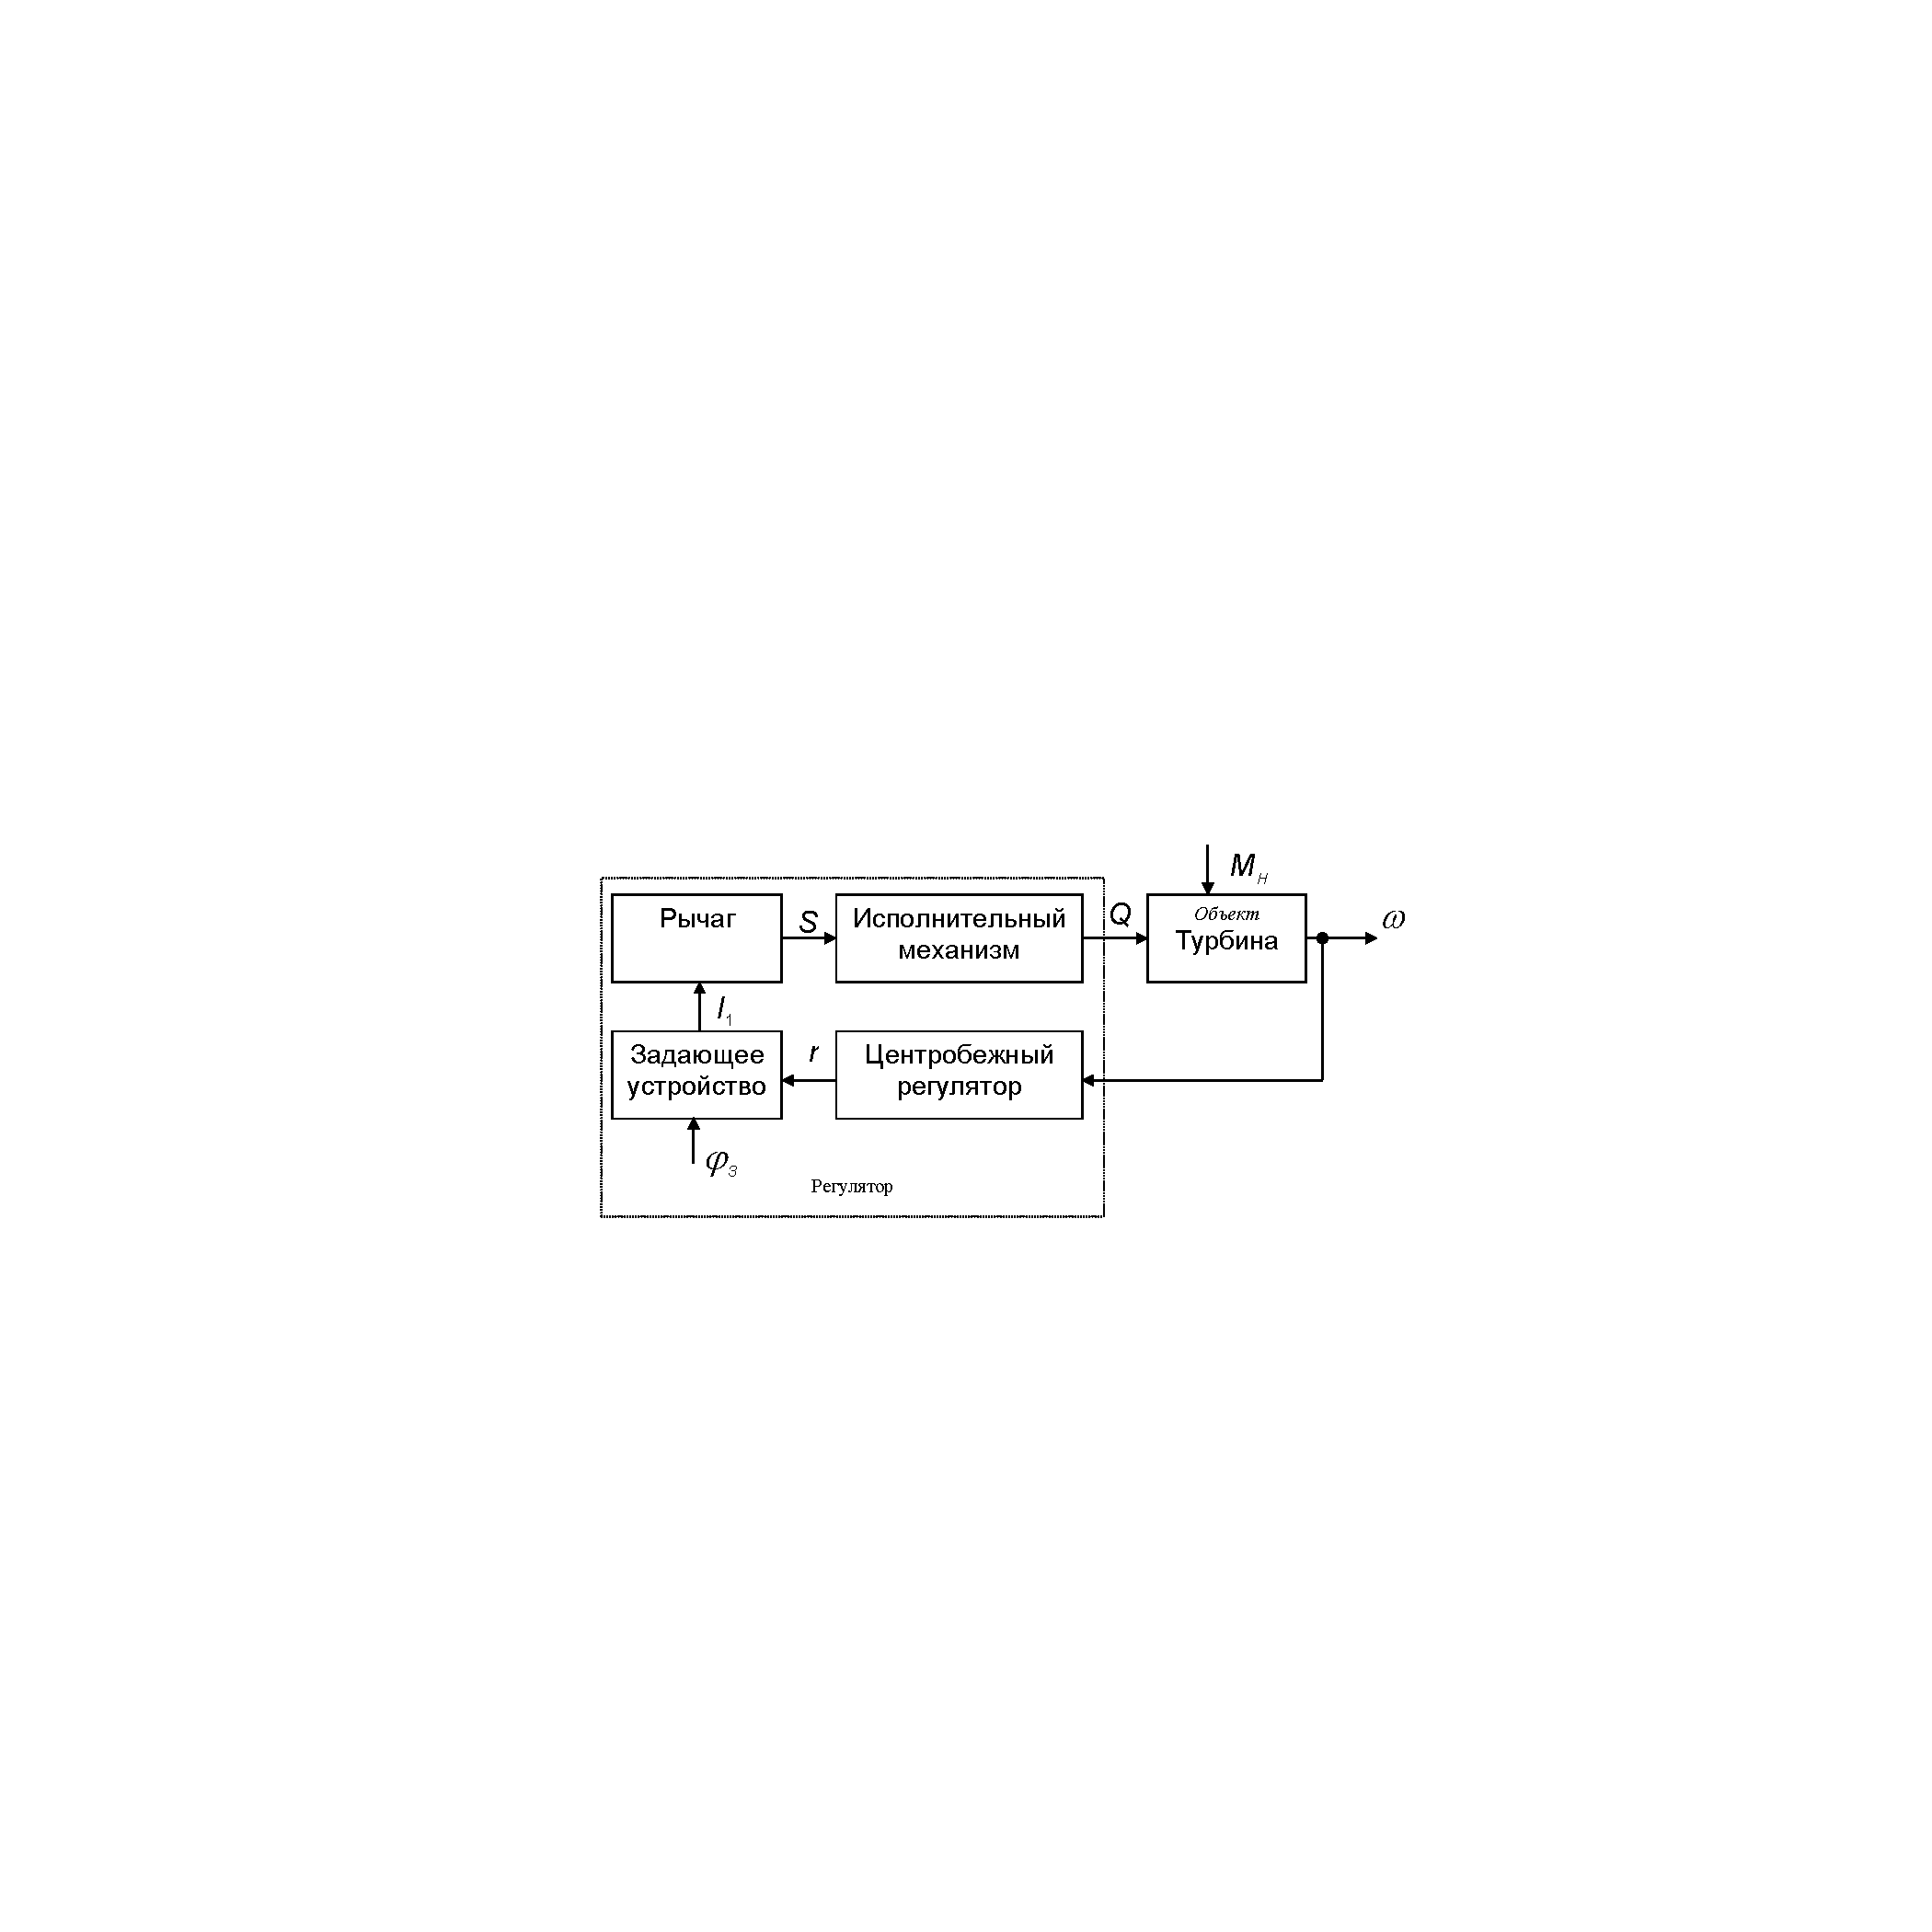
\includegraphics[scale=0.95]{images/FunctionStabilization}
	\caption{Функциональная схема системы стабилизации скорости турбины}
	\label{fig:functionstabilization}
\end{figure}

Типовая функциональная схема системы автоматического управления (САУ) представлена на рис.~\ref{fig:standardfunctionality},

где \begin{description}
		\item[$ u $---] управляющий сигнал;
		\item[$ y $---] управляемый сигнал;
		\item[f ---] возмущающее воздействие.
\end{description}

Кружок с четырьмя секторами является сумматором, причём сигнал, поступающий на зачернённый сектор, изменяет свой знак (вычитается).

\begin{figure}[h]
	\centering
	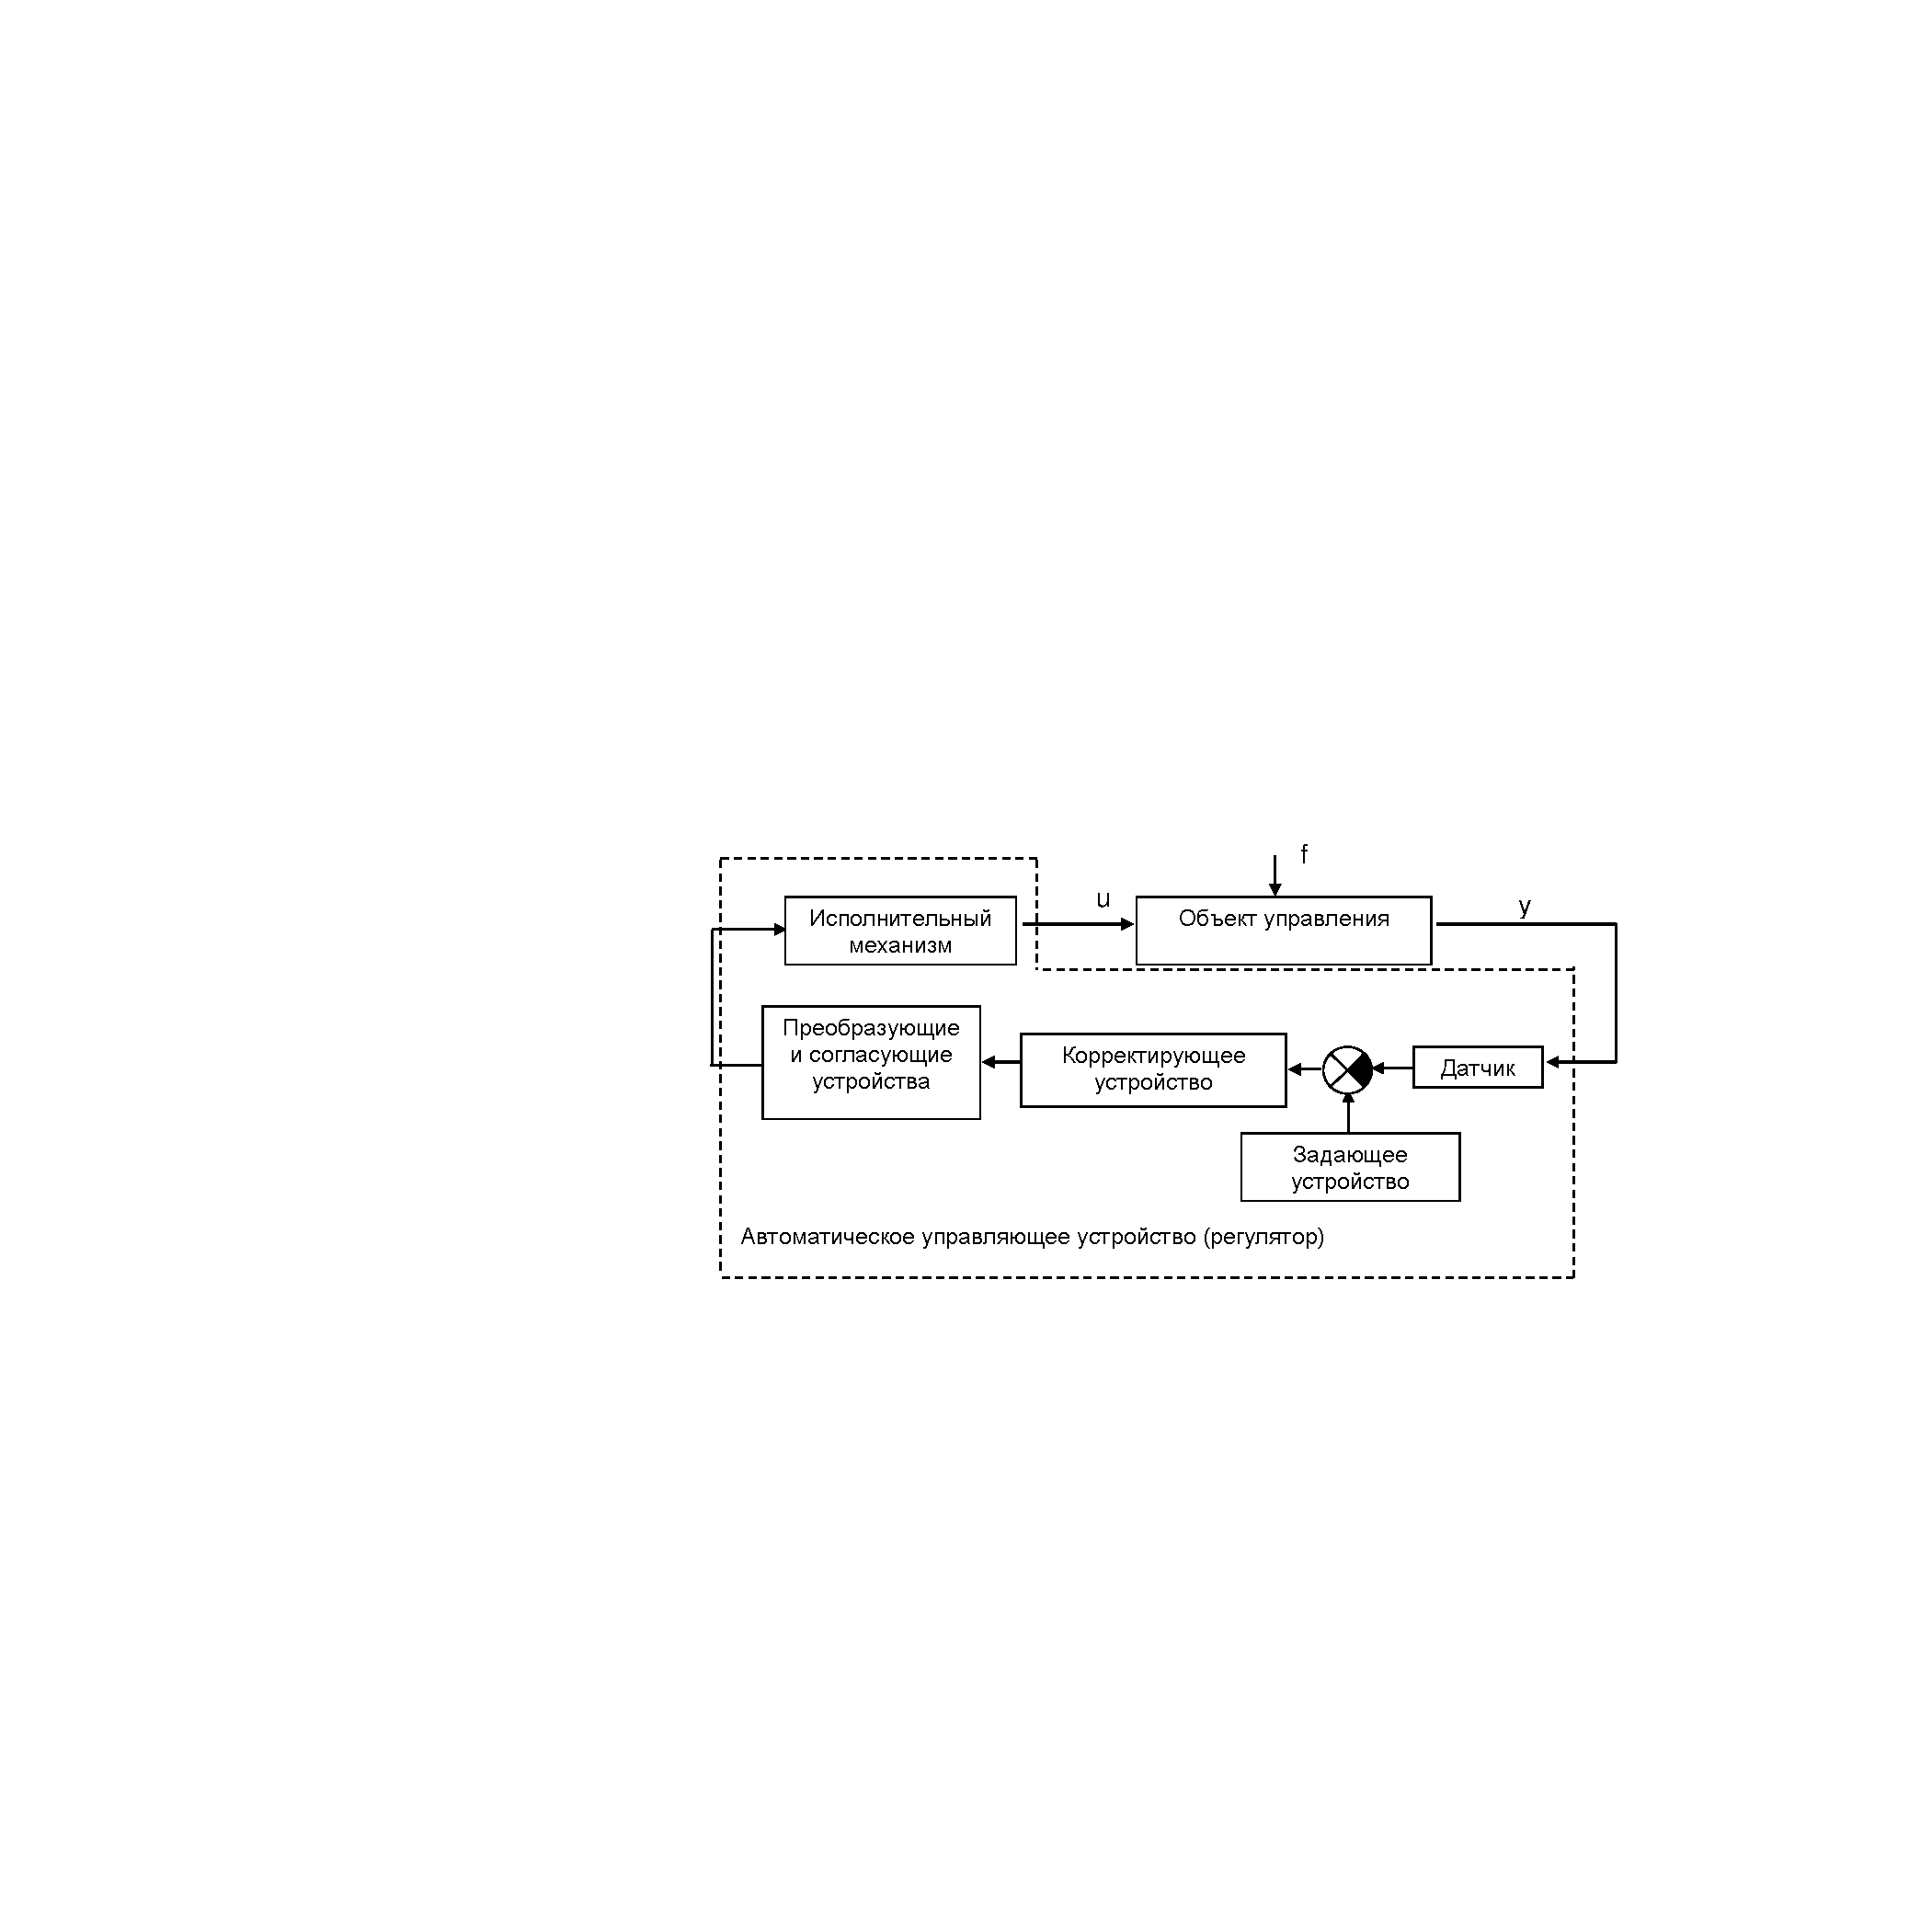
\includegraphics[scale=0.95]{images/Standardfunctionality}
	\caption{Типовая функциональная САУ}
	\label{fig:standardfunctionality}
\end{figure}

Рассмотрим вариант системы стабилизации скорости турбины, в котором сделана попытка устранить недостатки, 
присущие рассмотренной выше статической системе прямого действия. На рис.~\ref{fig:theturbinecontroller} показан регулятор для этой системы.

\begin{figure}[p]
	\centering
	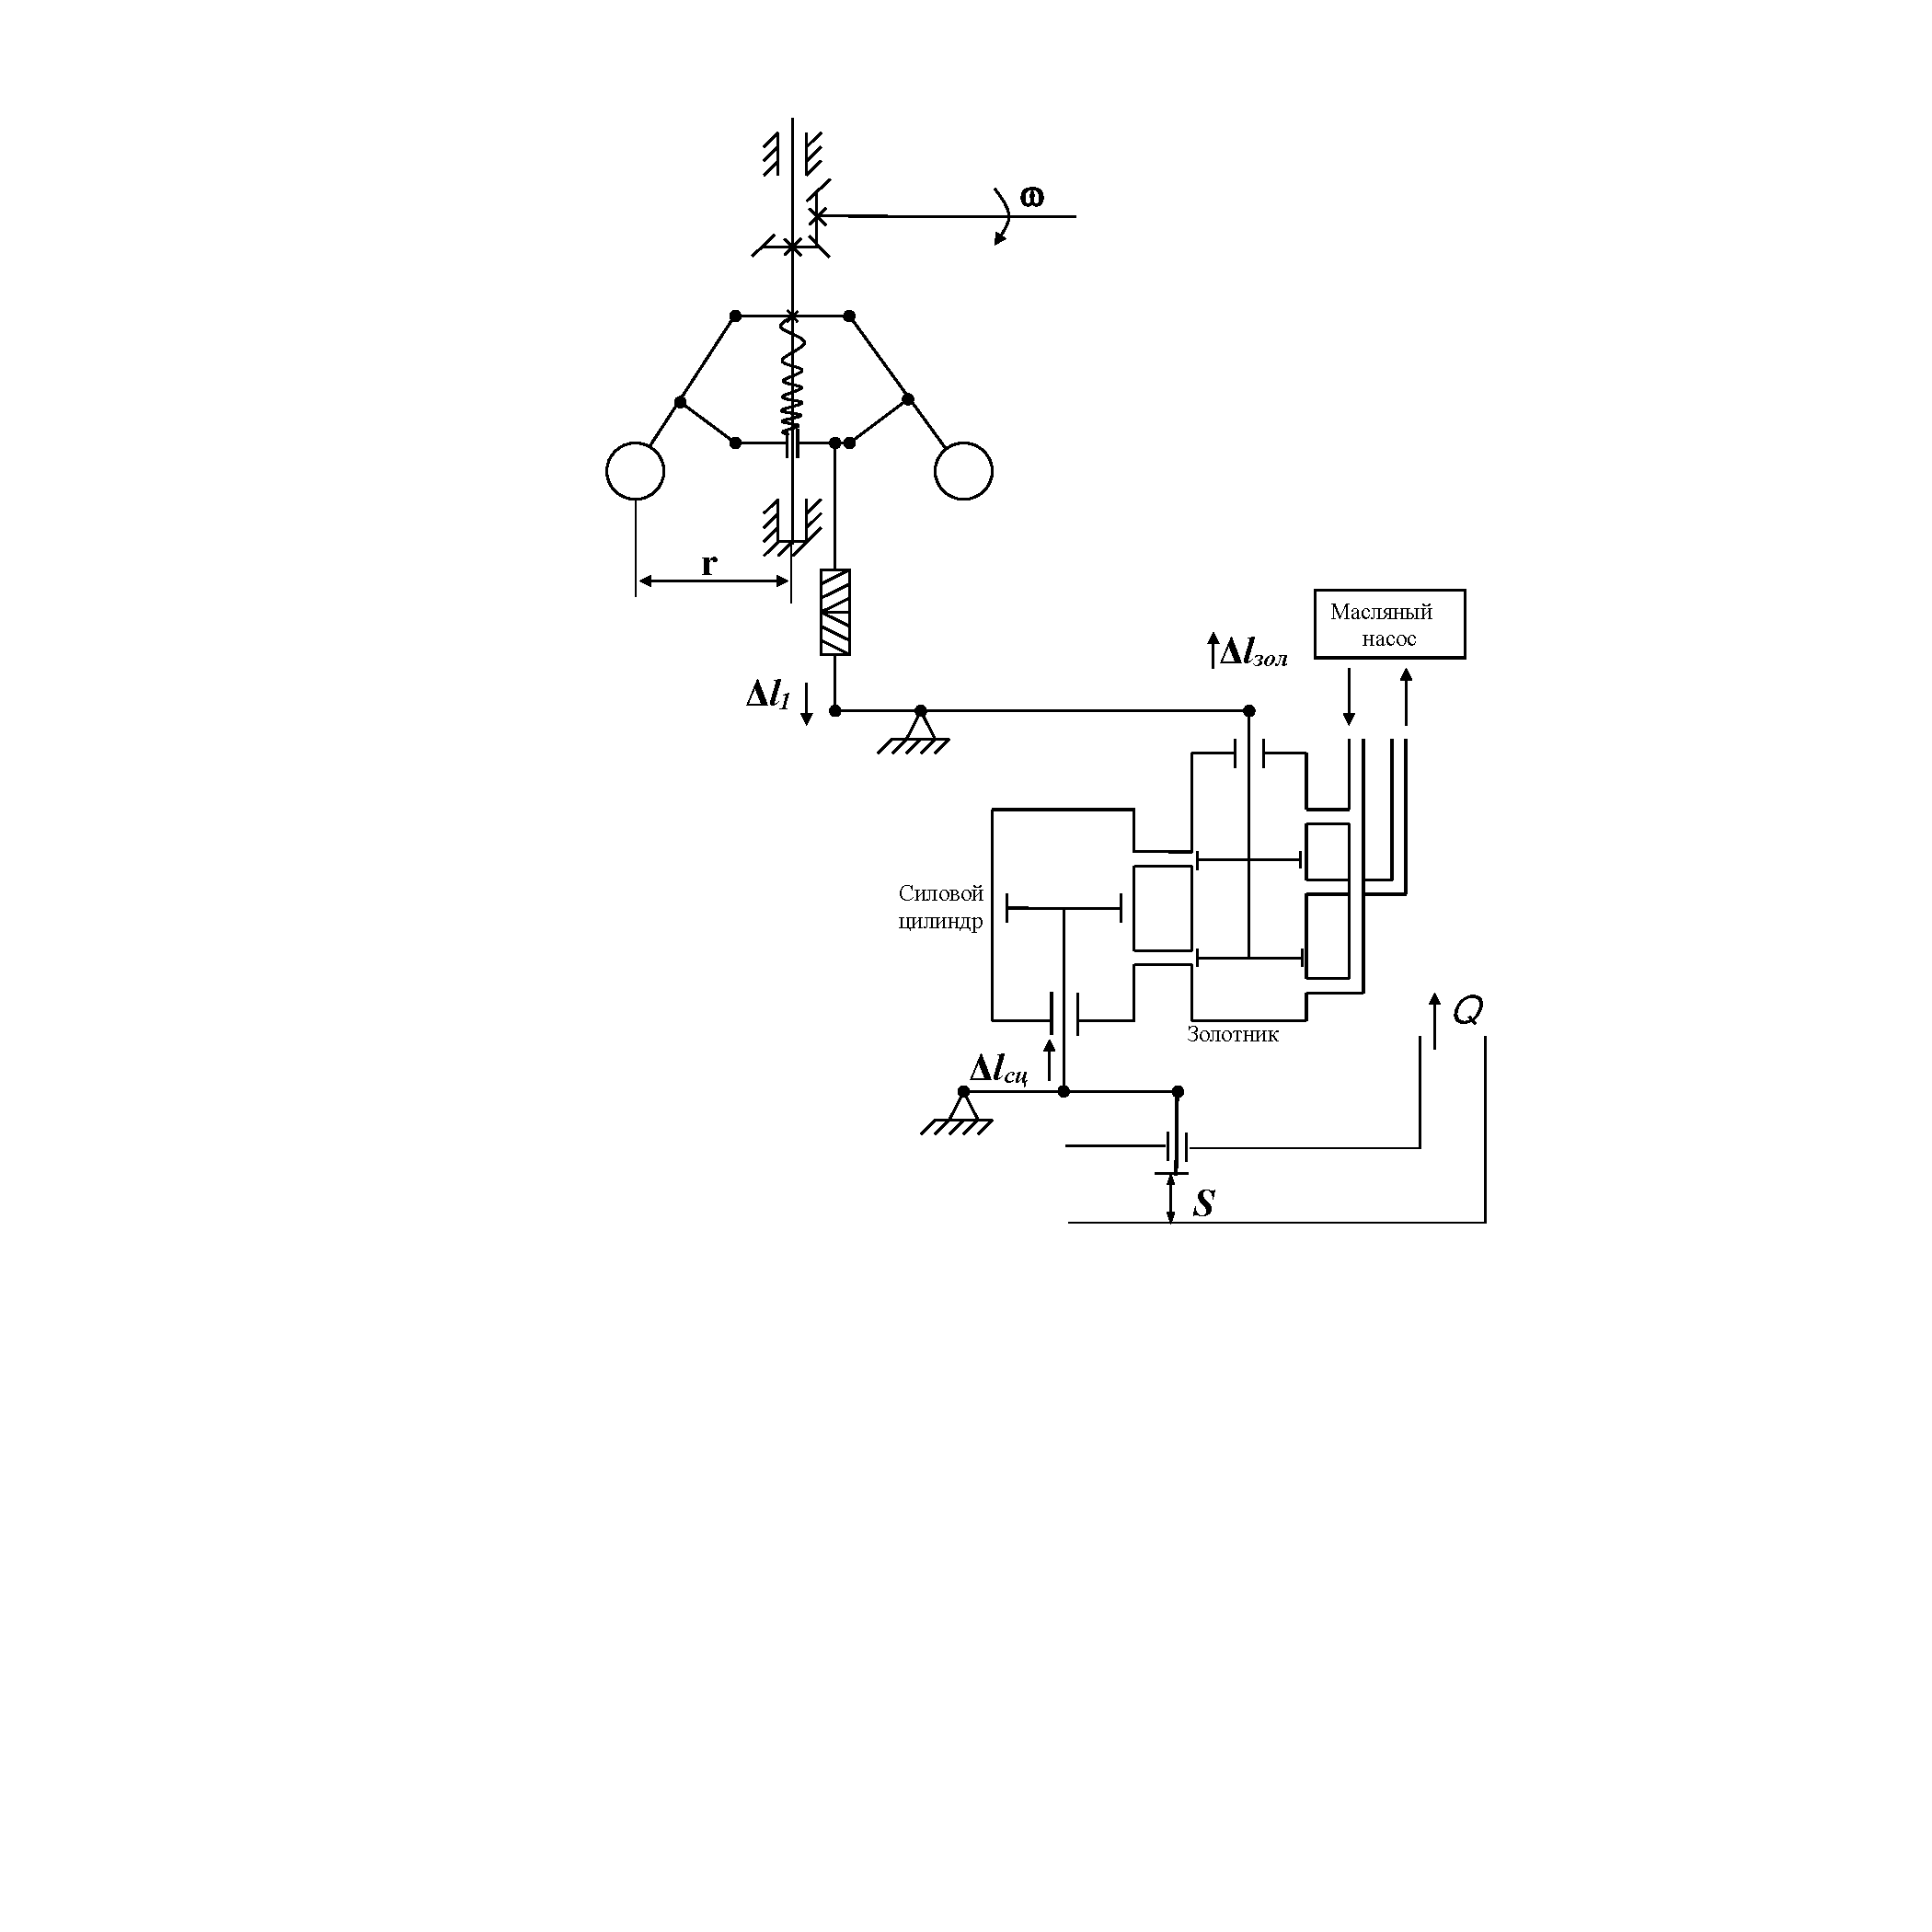
\includegraphics[scale=0.99]{images/TheTurbineController}
	\caption{Регулятор системы стабилизации скорости турбины 
		с использованием гидравлического усилителя}
	\label{fig:theturbinecontroller}
\end{figure}

Для этого в систему введен гидравлический усилитель, включающий в себя золотник, силовой цилиндр и масляный насос. Такая си-стема, в которой энергия регулятора потребляется от отдельного источника, называется \textit{системой непрямого действия}.

При заданной скорости расстояние между грузиками центробежного регулятора равно номинальному значению ($ r=r_{0} $), положение плеча золотника $ l_{зол} $ также равно номинальному значению $ (l_{зол}=l_{зол 0}) $ , при этом поршень золотника полностью перекрывает выходные отверстия, следовательно, положение поршня силового цилиндра неизменно.

С увеличением нагрузочного момента $ M_{Н} $ падают обороты турбины $ \omega $, что приводит к уменьшению расстояния $ $
между грузиками центробежного регулятора. В результате изменяет-ся положение поршенька золотника. Это, в свою очередь, приводит к перемещению поршня силового цилиндра, а следовательно, и к дополнительному приоткрытию заслонки $ S $.Соответственно увеличивается расход пара, возрастает скорость оборотов турбины $ \omega $ и увеличивается расстояние $ r $. Статика (установившееся состояние) в системе возможна только тогда, когда
$ l_{2}=l_{2_{0}} $, то есть когда полностью перекрыты перепускные отверстия золотникового устройства.

Теоретически в этой системе статическая ошибка равна нулю, то есть данная система является \textit{астатической}. В ней отсутствует статическая связь между скоростью и положением заслонки.

Рассмотрим упрощенные уравнения системы. Начнём с уравнения объекта. Очевидно, что изменение скорости турбины может про-исходить лишь в тех случаях, когда нарушается равновесие между движущим моментом турбины $ M_{Т} $и моментом нагрузки $ M_{Н} $:
\begin{equation}\label{eq:ObjectTurbine}
J\cfrac{d\Delta\Omega}{dt}=\Delta M_{Т}-\Delta M_{Н}
\end{equation}
где $ J $ --- суммарный момент инерции, приведённый к валу турбины.

С целью упрощения в уравнении (\ref{eq:ObjectTurbine}) использованы приращения скорости и моментов. Более подробно такой подход будет рас-смотрен в разделе, посвященном линеаризации систем.

Будем полагать, что приращение момента турбины пропорционально приращению количества подаваемого пара
\begin{equation*}
	\Delta M_{Т}=K_{Т}\Delta Q
\end{equation*}



Запишем уравнение центробежного регулятора. Полагая, что сами отклонения скорости и вызванные ими приращения внутренних переменных регулятора малы, мы можем выразить все зависимости в линейном виде. Тогда приращения скорости раскрытия грузиков и изменение положения поршенька золотника будут связаны линейными зависимостями: 
\begin{align}\label{eq:centrifugalController}
	&\Delta r=K_{\omega}\cdot\Delta\omega~;\\\nonumber
	&\Delta l_{зол}=-K_{r}\cdot\Delta r.
\end{align}

Составляя уравнение гидравлического усилителя, учтём, что скорость перемещения поршня силового цилиндра пропорциональна величине открытия перепускных отверстий золотника, то есть приращению $ l_{зол} $:

\begin{equation}\label{eq:hydraulic}
	\frac{d\Delta l_{сц}}{dt}=K_{зол}\cdot\Delta l_{зол}.
\end{equation}

Приращение координаты штока силового цилиндра повлечет за собой изменение положения заслонки и, следовательно, изменение количества подаваемого в турбину пара:	

\begin{equation}\label{eq:DeltaQ}
	\Delta Q=K_{сц}\cdot\Delta l_{сц}.
\end{equation}

Продифференцировав уравнение (\ref{eq:DeltaQ}) и учитывая уравнения для центробежного регулятора (\ref{eq:centrifugalController}) и гидравлического усилителя (\ref{eq:hydraulic}), получим уравнение для регулятора:

\begin{equation}
	\frac{d\Delta Q}{dt}=-K_{р}\cdot\Delta\omega,
\end{equation}
где $ К_{р}=K_{сц}\cdot K_{Зол}\cdot K_{r}\cdot K_{\omega} $ --- коэффициент регулятора.

Запишем совместно уравнения объекта и регулятора

\begin{equation*}
	\begin{cases}
		\cfrac{d\Delta\Omega}{dt}=k_{q}\cdot\Delta-K_{Н}\cdot\Delta M_{н};\\
		\cfrac{d\Delta Q}{dt}=-K_{р}\cdot\Delta\omega,
	\end{cases}
\end{equation*}
продифференцируем первое уравнение и подставим в него второе: 
\begin{equation*}
\cfrac{d^{2}\Delta\omega}{dt^{2}}=K_{q}(-K_{р}\cdot\Delta\Omega)-K_{Н}\cfrac{d\Delta M_{Н}}{dt}~.
\end{equation*}
При условии постоянства нагрузки получаем уравнение свободного движения всей системы
\begin{equation}\label{eq:freedom}
	\cfrac{d^{2}\Delta\omega}{dt^{2}}+K\cdot\Delta\omega=0,
\end{equation}
где
\begin{equation*}
	K=K_{р}\cdot K_{q}.
\end{equation*}
Соответствующее характеристическое уравнение имеет вид 
\begin{equation*}
	\lambda^{2}+K=0,
\end{equation*}
его корни - $ \lambda_{1,2}=\pm j\sqrt{K}, $

Таким образом, решение уравнения (\ref{eq:freedom}) имеет вид
\begin{equation}\label{eq:undampedOscillations}
	\Delta\omega(t)=C_{1}e^{\lambda_{1}t}+C_{2}e^{\lambda_{2}t}=A\sin(\sqrt{K}\cdot t+\varphi),
\end{equation}
где $ A \text{ и } \varphi $ определяются начальными условиями.

В результате решения получили, что в данной системе в принципе не существует установившегося (статического) состояния. Следовательно, система неработоспособна.

С целью успокоения незатухающих колебаний (\ref{eq:undampedOscillations}) введём в си-стему демпфер (рис.~\ref{fig:thesystemcontrollers}) и рассмотрим, что в ней происходит при изменении нагрузки. С увеличением нагрузочного момента $ M_{Н} $ уменьшается скорость вращения турбины $ \omega $, что приводит 
к уменьшению расстояния $ r $ между грузиками центробежного регулятора. Это влечет за собой изменение положения поршенька золотника $ \Delta l_{зол} $, а следовательно, и изменение положения поршня силового цилиндра. При этом одновременно происходит два процесса.

Во-первых, вместе со штоком силового цилиндра опускаются поршень и цилиндр демпфера, уменьшая первоначальное изменение $ \Delta l_{зол} $. Скорость перемещения поршня демпфера относительно его цилиндра невелика и регулируется с помощью специального дросселя Др.

Во-вторых, приоткрывается заслонка, увеличивая количество подаваемого в турбину пара, и начинает расти скорость $ \omega $.

За счёт первого движения поршни золотника могут перекрыть перепускные отверстия ещё до восстановления номинального значения $ \omega $. В то же время пружины стремятся вернуть демпфер в исход-ное положение, и, в конечном итоге, $ \Delta l_{2} $ стремится к нулю. Теперь уже перепускные отверстия золотника будут перекрыты только при номинальной скорости. Следовательно, система с демпфером, как и предыдущая, является астатической.
Рассмотрим, как повлияло введение демпфера на незатухающие колебания, выявленные в предыдущем варианте системы. Считая отклонения от номинального режима малыми, запишем уравнения эле-ментов регулятора. Как и раньше,
%Изменил, так вроде лучше выглядит
\begin{align}
	&\Delta r=K_{\omega}\Delta\omega,\\\nonumber
	&\Delta l_{1}=-K\cdot\Delta r;\\
	&	\cfrac{d}{dt}l_{сц}=K_{зол}\Delta l_{зол}.\label{eq:3eq}
\end{align}
%\begin{equation}
%
%\end{equation}

\begin{figure}[p]
	\centering
	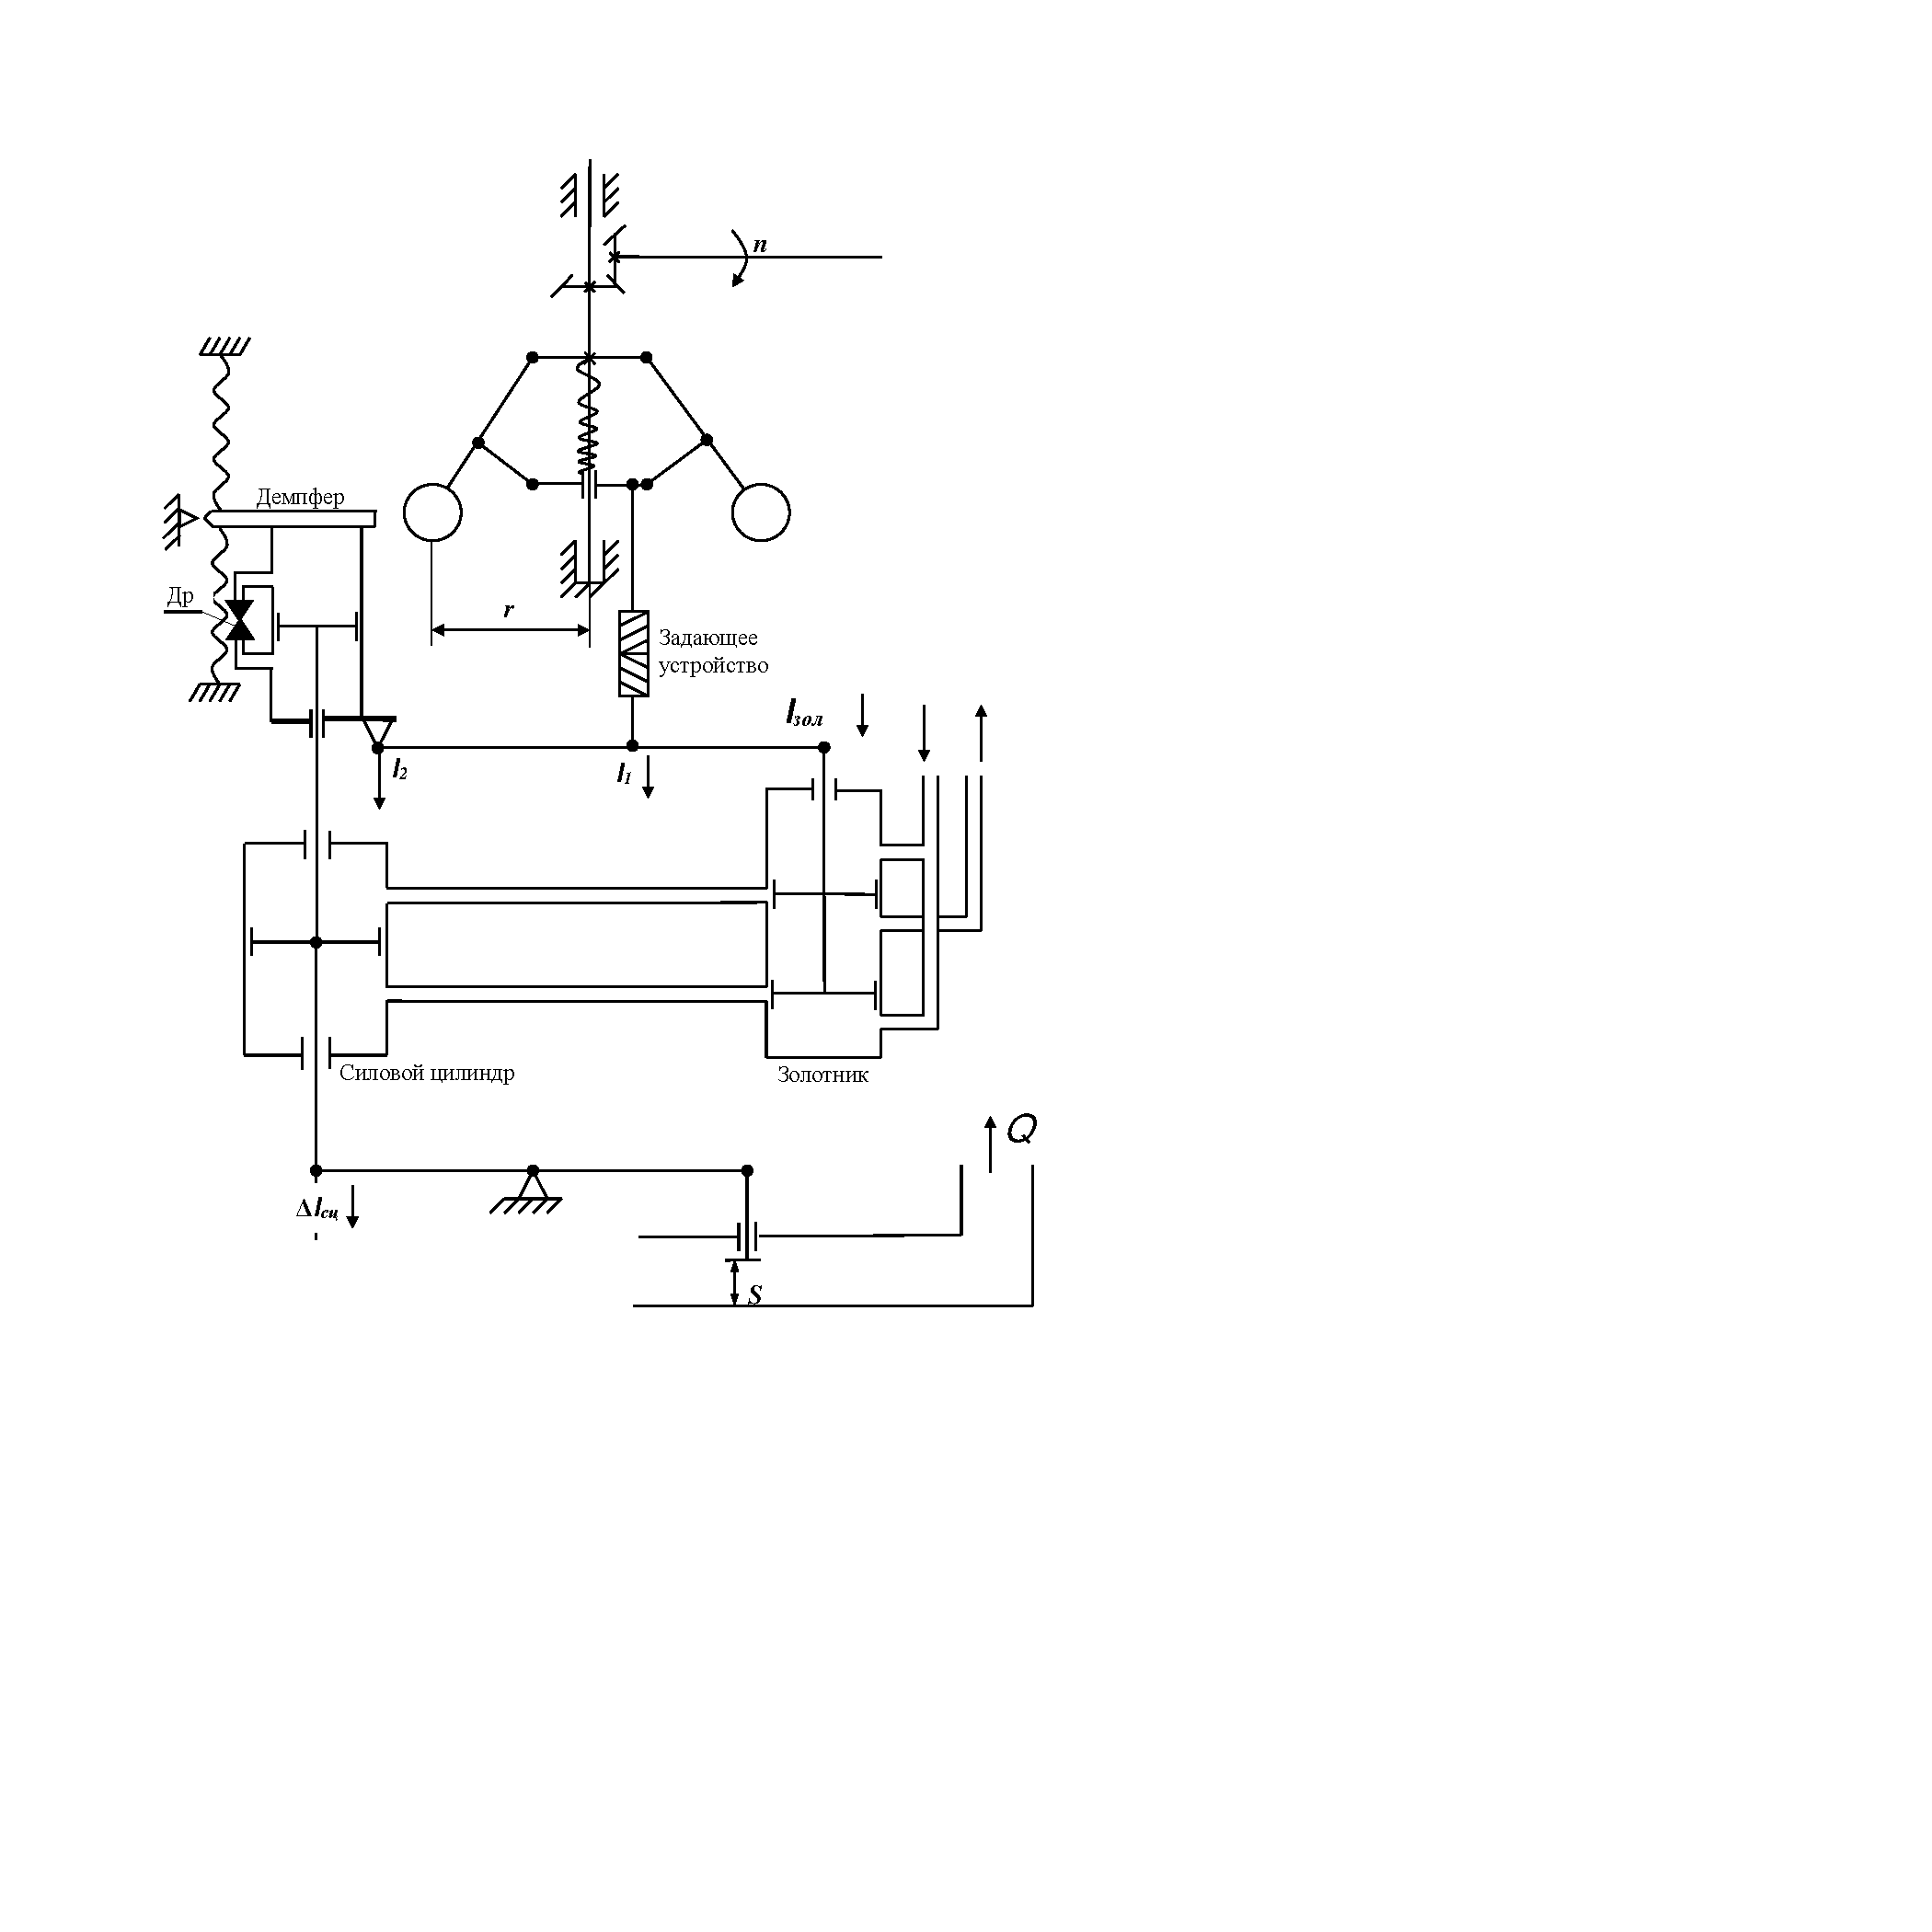
\includegraphics[scale=0.99]{images/TheSystemControllers}
	\caption{Регулятор системы стабилизации скорости турбины 
		с использованием успокоительного демпфера}
	\label{fig:thesystemcontrollers}
\end{figure}

В отличие от предыдущей системы, в данном случае положение штока золотника зависит не только от центробежного регулятора, но и от демпфера:
\begin{equation}\label{eq:PistonRod}
	\Delta l_{зол}=K_{1}\cdot\Delta l_{1}-K_{2}\cdot\Delta l_{2}.
\end{equation}
Упрощенные уравнения демпфера основываются на равенстве сил пружин:
%TT Что то тут не так 
\begin{equation*}
	\Delta F_{пр}=K_{пр}\cdot\Delta l_{2}.
\end{equation*}
и сил, связанных с перемещением поршня демпфера относительно корпуса:

\begin{equation*}
	F_{д}=k_{д}\cfrac{d(l_{сц}-l_{2})}{dt},
\end{equation*}
или
\begin{equation*}
	\frac{K_{д}}{K_{пр}}\cdot p\Delta l_{2}=\cfrac{K_{д}}{K_{пр}}\cdot p\Delta l_{сц}.
\end{equation*}
Таким образом, изображения перемещений штока силового цилиндра и корпуса демпфера связаны соотношением
\begin{equation}
	\Delta l_{2}=\cfrac{T_{д}p}{Т_{д}p+1}\cdot\Delta l_{сц},
\end{equation}
где постоянная времени демпфера
\begin{equation*}
	T_{д}=K_{д}/К_{пр}.
\end{equation*}
Из (\ref{eq:3eq}) и (\ref{eq:PistonRod}) следует
\begin{equation}
	
\end{equation}

